\documentclass[a4paper, 11pt, titlepage]{article}
\usepackage{graphicx}
\usepackage{subcaption}
%\usepackage{nath}
%\usepackage{gensymb}
\usepackage{indentfirst}




\usepackage{tikz}
\usepackage{circuitikz}

\addtolength{\hoffset}{-1.5cm}
\addtolength{\textwidth}{3cm}

\begin{document}
\title{EE568 Project 3: PM Motor Comparison Analysis}
\author{Baris Kuseyri}
\date{\today}
\maketitle

\pagenumbering{arabic}
\tableofcontents
\newpage

\section{Introduction}
\label{sec:intro}

In this assignment you are going to design several surface-mount PM machines with the following constant parameters:

Surface-mount permanent magnet (SPM) topology is kind of a machine where PMs mounted on the rotor surface, facing to the airgap \cite{hanselman}.


This project aims to prepare a study similar to what was done by W. L. Soong in his case study on Ferrite versus NdFeB. In his study, Soong replaces rare earth NdFeB magnets with ferrite magnets in an SPM machine. Later, he increases the thickness of the magnets and equalizes the flux density levels on stator tooth and back iron region of the machine with NdFeB magnets and ferrite magnets. Unlike Soong's study, this project sets the stator outer diameter constant.

First, this project designs a SPM in part \ref{sec:Q1}, to analyse the magnetic loading of a machine. Then, in part \ref{sec:Q2}, it determines several machine parameters. The project continues by analysing electric loading of the machine, and the resulting average tangential stress, total force, torque and power output.




This project aims to optimize a SPM machine, in which neodymium magnets. 

This project 

The starting values are given in Table \ref{table:machineParameters}, below.

\begin{table}[ht]
	\begin{center}
		\begin{tabular}{c|c|c|c}
			 & symbol & unit & value \\
			\hline
			number of phases & $m$ & & 3 \\
			number of pole-pairs & $p$ & & 2 \\
			motor axial length & $l_m$ & mm & 100 \\ 
			air-gap clearance & $\delta_g$ & mm & 1 \\
			magnet to pole pitch ratio & & & 0.8 \\
			magnet radial thickness & $t_m$ & mm & 4 \\
			\hline
		\end{tabular}
	\end{center}
	\caption{Machine Parameters}
	\label{table:machineParameters}
\end{table}
	


\section{Q1- Magnetic Loading}
\label{sec:Q1}

This project starts by analysing the magnetic loading of an SPM machine. The stator is assumed to be solid for this part. Additional to the parameters given in Table \ref{table:machineParameters}, some extra values are set as starting values. Parameters on rare earth magnet are given in Table \ref{fig:PMParameters} and rotor diameter is given in Table \ref{table:rotorParameter}.





\begin{table}[h]
	\begin{center}
		\begin{tabular}{c|c|c|c}
			 & symbol & units & value \\
			\hline
			magnet type & & & NdFeB N42 \\
			shape & & & radial \\ 
			relative permeability & $\mu_r$ & & 1.05 \\
			coercivity & $H_c$ & $A/m$ & 994529 \\
			\hline
		\end{tabular}
	\end{center}
	\caption{Permanent Magnet Parameters}
	\label{fig:PMParameters}
\end{table}


\begin{table}[h]
	\begin{center}
		\begin{tabular}{c|c|c|c}
			 & symbol & unit & value \\
			\hline
			rotor diameter & $D_r$ & mm & 100 \\
			\hline
		\end{tabular}
	\end{center}
	\caption{Rotor Dimensions}
	\label{table:rotorParameter}
\end{table}




\subsection{a. Magnetic Equivalent Circuit, Magnet Load Line and Peak Air-gap Flux Density}
\label{sec:peakAir-gapFluxDensity}

Magnetic equivalent circuit for one pole-pair is shown in Fig. \ref{fig:magneticCircuit}. Here, each PM is modelled as an MMF source, meaning it's equivalent model is composed of a voltage source with a value of $F=\phi R_m$, and a resistance $R_m$ connected in series.

Starting with PM \#1, the flux $\phi$ goes through the airgap, modelled as $R_g$, and splits into two components at the stator back iron. Each half of the flux goes through the back iron, in opposite directions. Here, only one pole-pair is shown, so only one half-of-the-flux is described further. This half flux component then merges with, again what is another half flux component, and travels through the airgap, modelled again as $R_g$. Then, it travels through PM \#2, and splits into two. One of the components merges with another half flux components and goes through PM \#1. Hence, the cycle is completed.

\begin{figure}[h]
	\begin{center}
		\begin{circuitikz}
			\draw (0,0)
			to[short,i_=$\frac{\phi}{2}$,*-*] (0,2)
			to[short,i_=$\phi$,*-*] (1,2)
			to[battery,l^=$F$, invert,*-] (2,2)
			to[R=$R_m$,i_=$\phi$,-*] (5,2)
			to[R=$R_g$] (7,2)
			to[short,i_=$\phi$] (8,2)
			to[short,i_=$\frac{\phi}{2}$,*-*] (8,0)
			to[short,i_=$\phi$] (7,0)
			to[R=$R_g$] (5,0)
			to[battery,l^=$F$, invert,*-] (4,0)
			to[R=$R_m$,i_=$\phi$,-*] (1,0)
			to[short,i_=$\phi$] (0,0);
			\draw (0,4)
			to[short,i_=$\frac{\phi}{2}$] (0,2);
			\draw (8,2)
			to[short,i_=$\frac{\phi}{2}$] (8,4);
			\draw (8,-2)
			to[short,i_=$\frac{\phi}{2}$] (8,0);
			\draw (0,0)
			to[short,i_=$\frac{\phi}{2}$] (0,-2);
			\draw[black, thick] (1,1.5) rectangle (5,3.5)
			node[pos=0.5, above=10pt]{PM \#1};
			\draw[black, thick] (1,-1) rectangle (5,1)
			node[pos=0.5, above=10pt]{PM \#2};
		\end{circuitikz}
	\caption{magnetic equivalent circuit for one pole-pair}
	\label{fig:magneticCircuit}
	\end{center}
\end{figure}



Magnetic loading of a machine refers to the average airgao flux density over a pole. This value can be calculated by

\begin{equation}
	\bar{B}=\frac{p\phi_p}{\pi D_rl}
	\label{eq:specificMagneticLoading}
\end{equation}

where $\bar{B}$ is specific magnetic loading, $p$ is the number of poles, $\phi_p$ is flux per pole, $D_r$ is rotor diameter, and $l$ is the axial length of the machine. Equation \ref{eq:specificMagneticLoading} interprets specific magnetic loading $\bar{B}$ as total flux going out of the rotor surface divided by total rotor surface area.

To find out $\phi_p$, machine's magnetic circuit is needed to be analyzed. The magnetic circuit diagram can be seen in Fig. \ref{fig:magneticCircuit}. 

The magnetic circuit is composed of 2 NdFeB 42 permanent magnets (PM) and 2 instances of airgaps. To analyse this circuit, PM remanence flux density $B_r$ information is required. At this point, relative permeability $\mu_r$ and coercivity $H_c$ of NdFeB 42 PM is given as a part of the problem, which can be seen in Table \ref{fig:PMParameters}. From here; remanence flux density can be found by the following relation:

\begin{equation}
	B_r = \mu_0\mu_r\times H_c 
	\label{label:remanenceFluxDensity}
\end{equation}

where, $\mu_0$ is the permeability of air or vacuum ($\mu_0=4\pi \times 10^{-7}A/m$). Hence, magnet remanence flux density  is $B_r=1.31 T$. Now,



The values for airgap flux density $B_g$ Calculating peak airgap flux density 


\subsection{b. Magnetic Loading}
\label{sec:specificMagneticLoading}

The average airgap flux density $B_{avg}$ corresponds to the $RMS$ value of peak airgap flux density $\hat{B}_g$, which corresponds to specific magnetic loading $\bar{B}$ of the machine.

\begin{equation}
	B_{avg} = \frac{1}{\sqrt{2}}\hat{B}_g = \bar{B}
	\label{eq:specificMagneticLoading}
\end{equation}

Peak airgap flux density $\hat{B}_g$ is calculated in the previous section, and the result is $1.0394T$. Inserting this value to the Eq. \ref{eq:specificMagneticLoading}, specific magnetic loading is $\bar{B}=0.7350T$.


\subsection{c. FEA Results}

FEMM is used as FEA software. The flux density map of the machine is shown in Fig. \ref{fig:Bmap}. The stator is solid, meaning that there is no tooth apparent on the stator.

The airgap flux density $B_g$ distribution can be seen in Fig. \ref{fig:airgapBplot}. The distribution peaks at a value of $\hat{B}_g = 1.0374T$. Specific magnetic loading is calculated by taking the average of this distribution, which results with $B_{avg}=0.7558T$.

\begin{figure}[h]
	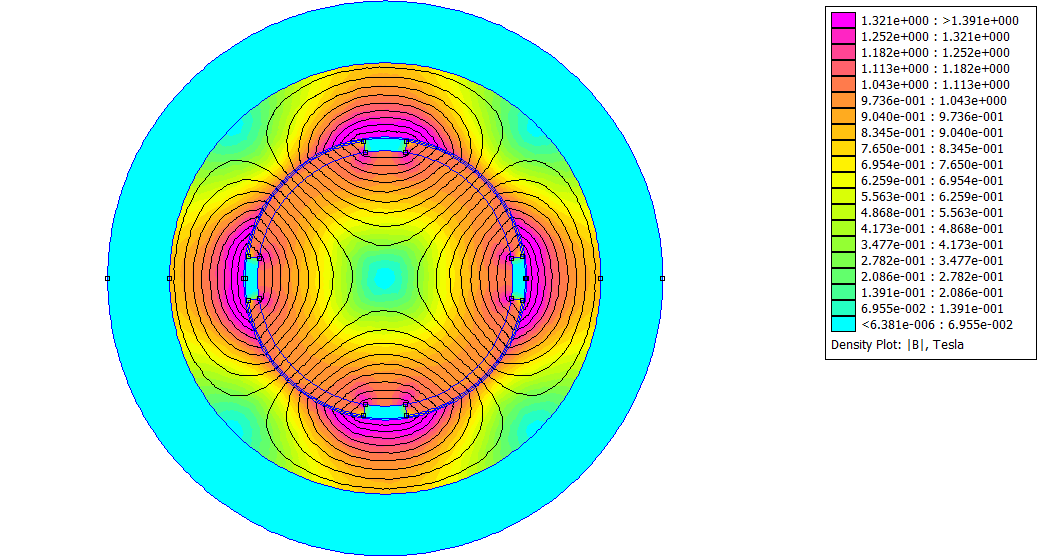
\includegraphics[width=\textwidth]{fluxDensity.png}
	\caption{Flux Density Plot}
	\label{fig:Bmap}
\end{figure}

\begin{figure}[h]
	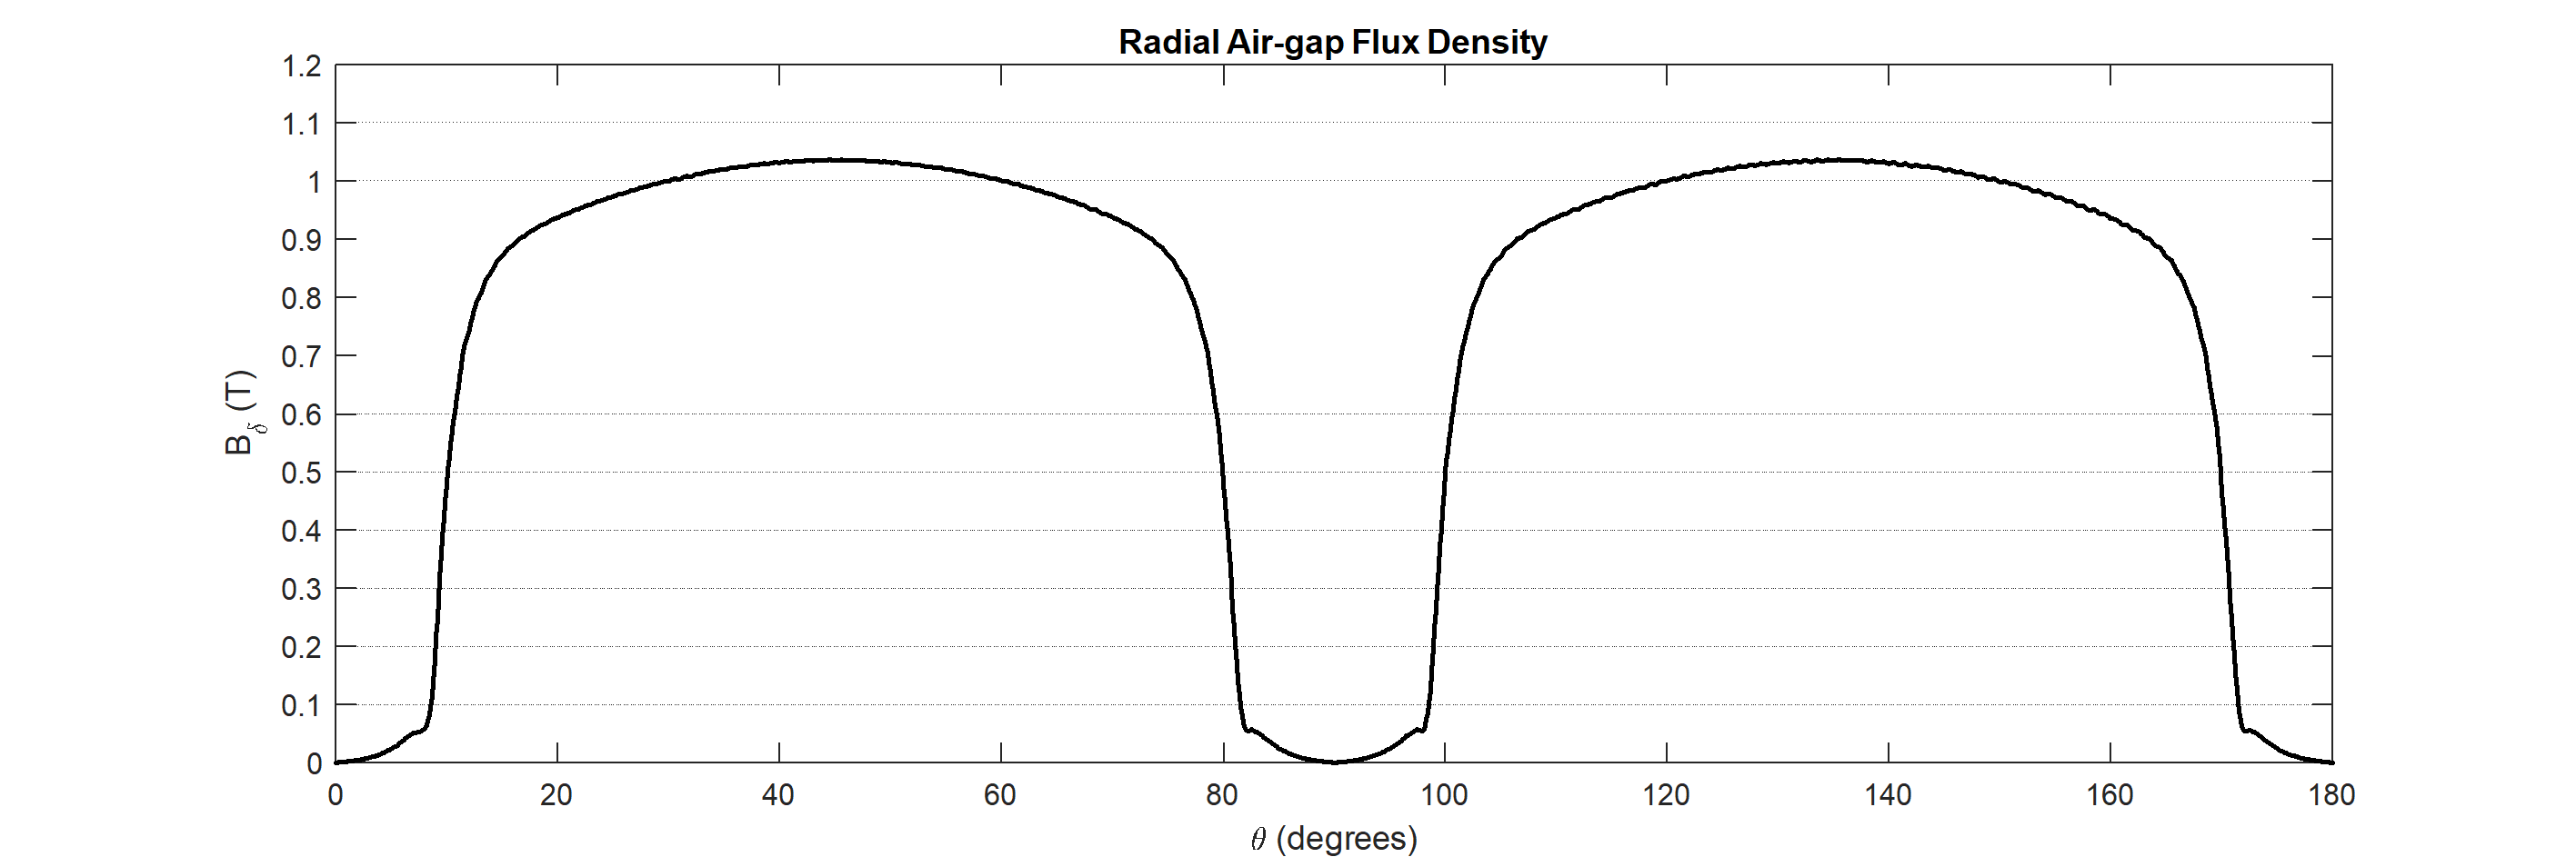
\includegraphics[width=\textwidth]{airgapFluxDensity.png}
	\caption{Airgap Flux Density Distribution}
	\label{fig:airgapBplot}
\end{figure}

Analytical and FEA results for peak airgap flux density $\hat{B}_g$ and magnetic loading $\bar{B}$ are shown in Table \ref{fig:BpeakandBavg}.

\begin{table}[h]
	\begin{center}
		\begin{tabular}{c|c|c}
			 &  $\hat{B}_g$ & $\bar{B}$ \\
			\hline
			Analytic & $1.0394T$ & $0.7350T$ \\
			\hline
			FEA & $1.0374T$ & $0.7558T$ \\ 
			\hline
		\end{tabular}
	\end{center}
	\caption{Peak Airgap Flux Density and Magnetic Loading}
	\label{fig:BpeakandBavg}
\end{table}

Results obtained in pervious sections \ref{sec:specificMagneticLoading} and \ref{sec:peakAir-gapFluxDensity} comply with the results from FEA analysis. Error calculation, according to Appendix \ref{app:errorCalculation}, yields a $0.1977\%$ error for the peak airgap flux density $\hat{B}_g$ between the analytical and FEA results. Same calculation yields a $2.7518\%$ error for the magnetic loading $\bar{B}$ between the analytical and FEA results, slightly higher than it is for peak airgap flux density $\hat{B}_g$; however, both error percentages are fairly small. Overall, the FEA results verify the analytical results.

\section{Q2- Electrical Loading \& Machine Sizing}
\label{sec:Q2}

\subsection{a. Number of Slots}

This project studies machine topologies with a number of pole-pairs of $p=2$. Number of slots for this machine is determined to be 12. In a 12 slot 4 pole machine, fundamental winding factor is unity, meaning the windings link all the flux components coming from the magnets.

Several slot numbers $N_s$ and the corresponding winding factors $K_w$ are given in Table \ref{fig:NsvsKw}.

\begin{table}[h]
	\begin{center}
		\begin{tabular}{c|c|c}
			number of slots $N_s$ & winding factor $K_w$ & winding type \\
			\hline
			$6$ & $0.866$ & concentrated \\
			\hline
			$9$ & $0.617$ & concentrated \\
			\hline
			$12$ & $1.000$ & integer-slot \\
			\hline
			$15$ & $0.951$ & fractional-slot \\
			\hline
			$18$ & $0.945$ & fractional-slot \\
			\hline
		\end{tabular}
	\end{center}
	\caption{Number of Slots and Corresponding Winding Factors}
	\label{fig:NsvsKw}
\end{table}

One major downside of this is that there is high EMF harmonic components. Another downside is the resulting high cogging torque.

\subsection{b. AWG Cable}

\begin{table}[h]
	\begin{center}
		\begin{tabular}{c|c|c|c}
			 & symbol & units & value \\
			\hline
			max. current density & $J$ & $A/mm^2$ & 5 \\
			coil current & $I$ & A & 2.5 \\ 
			fill factor & $K_p$ & & 0.6 \\
			\hline
		\end{tabular}
	\end{center}
	\caption{Permanent Magnet Parameters}
	\label{fig:PMParameters}
\end{table}


If the maximum current density $\hat{J}$ is set to be $5 A/mm^2$ and one conductor is carrying $2.5A$, then the maximum number of conductors there can be in $1mm^2$ is 2, and the total cross-section area of 2 conductors can not be below $1mm^2$. Therefore, the suitable AWG cable chosen for this project is AWG 20. The characteristics of AWG20 cable can be seen in Table \ref{tab:AWG20}, below.

\begin{table}[h]
	\begin{center}
		\begin{tabular}{c|c|c|c}
			AWG & diameter [$mm$] & area [$mm^2$] & resistance/length [m$\Omega$/m] \\
			\hline
			20 &  0.812 & 0.518 & 33.31 \\
			\hline
		\end{tabular}
	\end{center}
	\caption{AWG 20 characteristics}
	\label{tab:AWG20}
\end{table}


As can be seen in Table \ref{tab:AWG20}, the cross-section area of AWG 20 cable is $0.518mm^2$, which corresponds to $J=4.83A/mm^2$, below the maximum current density value given for this project. Using any cable with a cross-section area below $0.500mm^2$ with a coil current of $I=2.5A$ would exceed this current density $J$ limitation.


\subsection{c. Slot Height, Number of Coils per Slot, and Back-core Thickness}

This part starts by choosing a slot ratio $d$ for the machine. This choice is done in the following fashion. Teeth shape is determined to be rectangular. Then, the slot area is calculated by



where $A_s$ is slot area, $N_s$ is the number of slots, $r_{so}$ is the slot outer radius, $r_{si}$ is the slot inner or stator inner radius, and $A_t$ is the area of tooth.

First, tooth to slot opening ratio is assumed to be 1 to 1. Then, 

\begin{equation}
	\tau_{teeth} = \tau_{slot} = \frac{2\pi r_{si}}{2N_s}
\end{equation}

where $\tau_{teeth}$ is the tooth thickness and $\tau_{slot}$ is the slot opening. 

\begin{equation}
	h_t = \frac{r_{si}}{d}-r_{si}
\end{equation}

where $h_t$ is tooth height. Then, tooth area is calculated by

\begin{equation}
	A_t = h_t \tau_{teeth}
\end{equation}

\begin{equation}
	N_sA_s = (\pi r_{so}^2 - \pi r_{si}^2)-N_sA_t
\end{equation}

Hence, the slot area $A_s$ is calculated.

Then, the number of conductors to be fit in a slot is determined by

\begin{equation}
	N_{cond} = \frac{A_sK_p}{A_{cond}}
	\label{eq:numberOfConductorsPerSlot}
\end{equation}

Hence, the number of conductors to be fit in one slot is $N_{cond}=999$. 


\subsection{d. Electrical Loading}


Now that the number of conductors per slot is determined, the electric loading of the machine can be calculated.

\begin{equation}
	\hat{A} = \frac{N_sN_{cond}I}{2\pi r_{si}}\frac{1}{\sqrt{2}}
	\label{eq:specificElectricLoading}
\end{equation}

\subsection{e. Average Tangential Stress \& Total Force}

\begin{equation}
	l'=l+2l_g
	\label{eq:effectiveAxialLength}
\end{equation}


\begin{eqnarray}
	\sigma_{tan} = \frac{\bar{A}\hat{B}}{\sqrt{2}} \\
	F = 2\sigma_{tan}\pi r_{r}l' \\
	T = Fr_{r}= 2\sigma_{tan}\pi r^2_{r}l'
	\label{eq:torqueOutput}
\end{eqnarray}

\subsection{f. Expected Power Output}

\begin{equation}
	P=T\times\omega
\end{equation}


\section{Q3- Comparison \& Optimization}

In this part, the stator outer diameter $D_o$ is set to be $160mm$, and rotor diameter $D_r$ and other parameters are subjected to alteration. Open slot configuration and rectangular teeth geometry is determined as starting parameters. 


\subsection{a. Optimum Rotor Diameter}
The aim of this part is to find the optimum rotor diameter and the slot ratio, which yields the maximum torque output. To achieve this, torque output is derived as a function of rotor radius. The derivation of electric loading as a function of rotor radius can be found in Appendix \ref{app:torquevsRotorRadius}. Then, tangential stress $\sigma_{Ftan}$ is calculated by

\begin{equation}
	\sigma_{Ftan}=\bar{A}\bar{B}
	\label{eq:tangentialStress}
\end{equation}

Here, tangential stress acting on every point on the rotor surface. Thus, integrating the tangential stress over rotor surface yields the total force $F_{tan}$ acting on the rotor surface in the tangential direction.

\begin{eqnarray}
	F_{tan} &=& 2\sigma_{Ftan}V_r \\
	&=& 2\sigma_{Ftan}(\pi r^2_{rotor,outer}l_e)
	\label{eq:totalTangentialForce}
\end{eqnarray}

To obtain the torque $T$ equation, force $F_{tan}$ shown in Eq. \ref{eq:totalTangentialForce} is multiplied by the rotor outer radius $r_{rotor,outer}$.

\begin{equation}
	T=F_{tan}r_{rotor,outer}
	\label{eq:torqueOutput}
\end{equation}

Thus, the relationship between rotor outer radius $r_{rotor,outer}$ and the torque output $T$ is set. Additionally, slot ratio $d$ is stated as a function of rotor outer radius $r_{rotor,outer}$.


\begin{equation}
	d = \frac{r_{slot,inner}}{r_{slot,outer}}
	\label{eq:dvsRotorRadiusOuter}
\end{equation}

where, $r_{slot,inner}$ and $r_{slot,outer}$ are defined as functions of $r_{rotor,outer}$ in Appendix \ref{app:torquevsRotorRadius}. Thus, the relationship between slot ratio $d$ and the torque output $T$ is set.

Using MATLAB, torque output $T$ is plotted as a function of rotor outer radius $r_{rotor,outer}$, in Fig. \ref{fig:TvsD}.

\begin{figure}[h]
	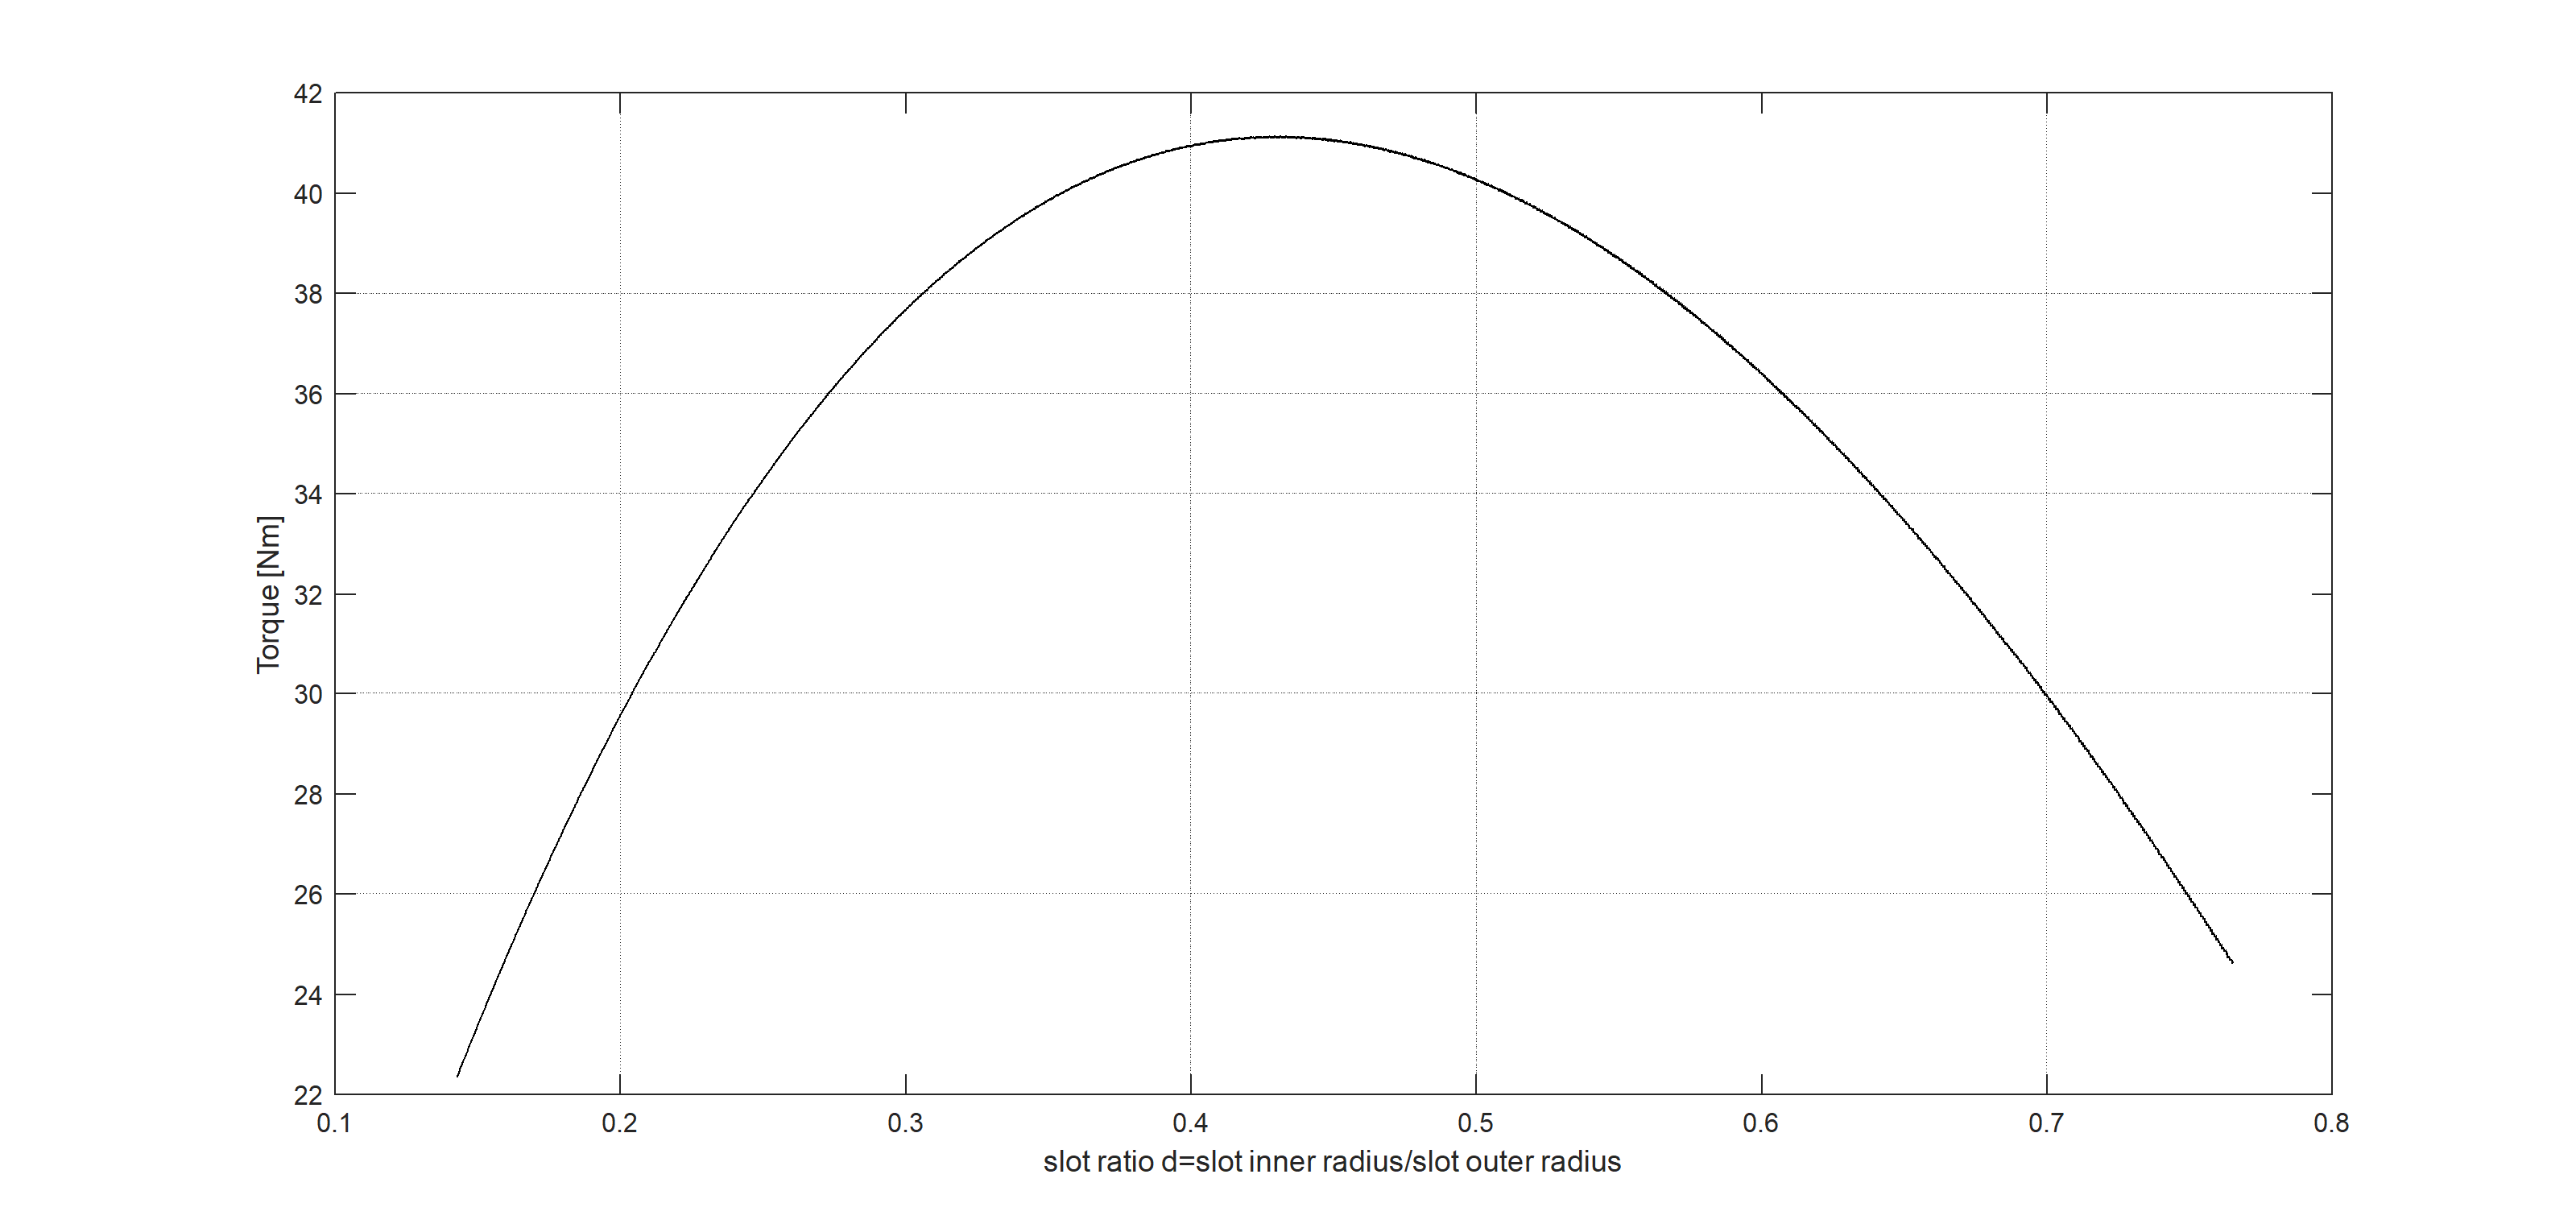
\includegraphics[width=\textwidth]{torquevsD_NdFeB.png}
	\caption{Torque vs. Slot Ratio}
	\label{fig:TvsD}
\end{figure}

The torque function peaks at slot ratio $d=0.4313$, with a torque value of $T=41.1443Nm$.


\subsection{b. Replacing NdFeB with Ferrite}

\begin{figure}[h]
	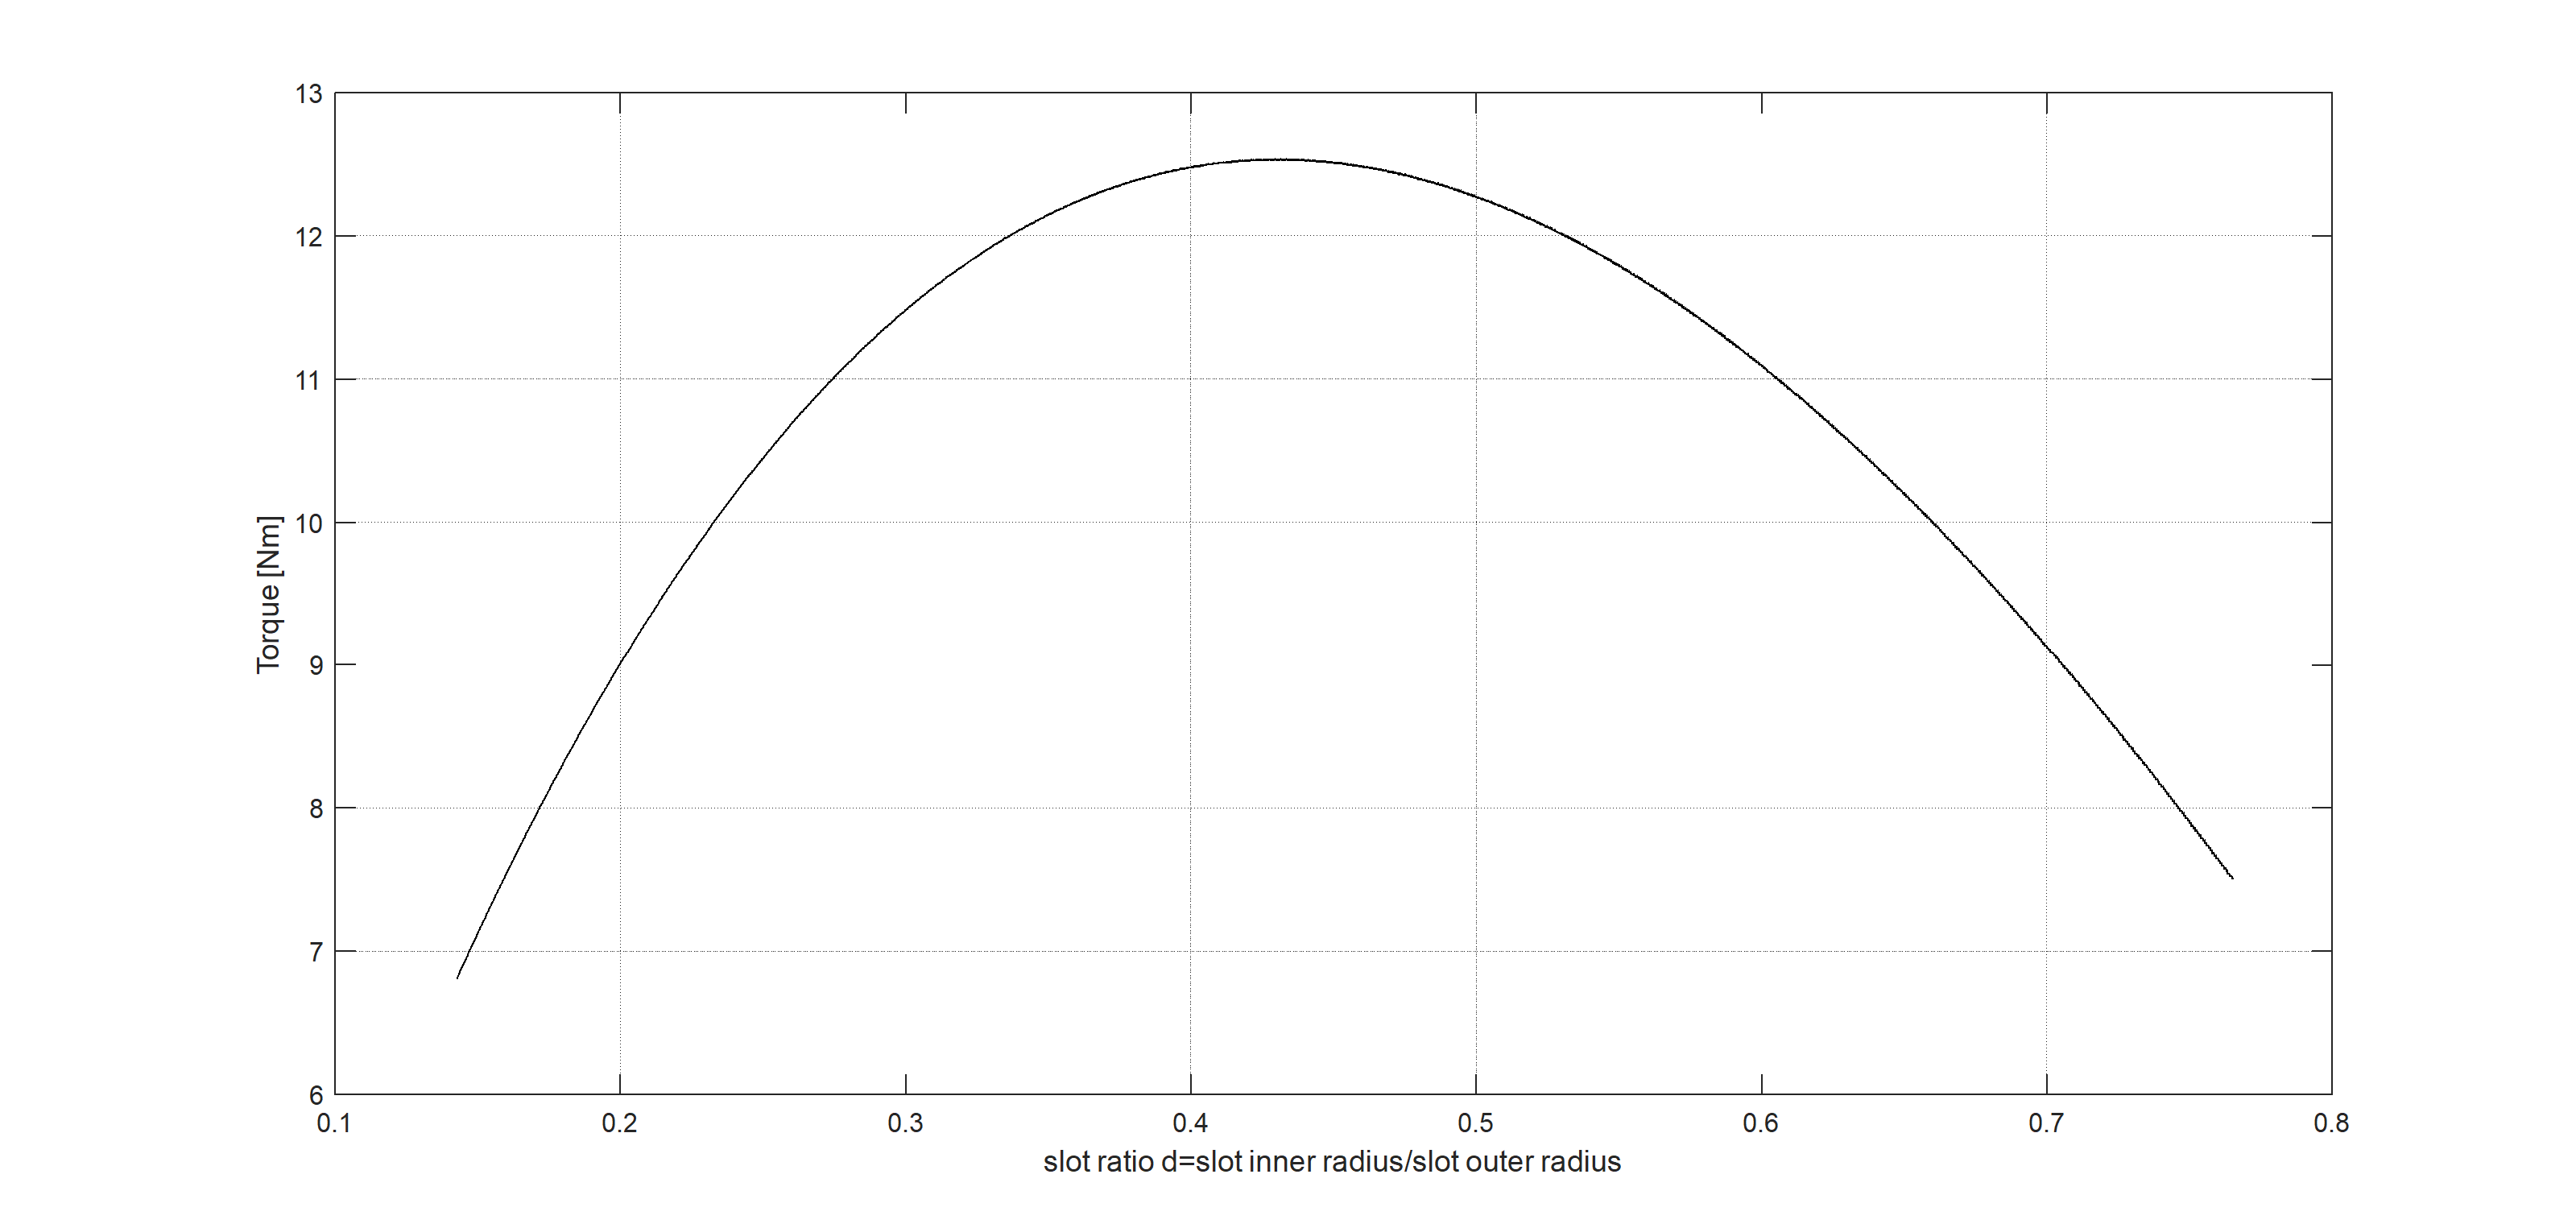
\includegraphics[width=\textwidth]{torquevsD_Ferrite.png}
	\caption{Torque vs. Slot Ratio}
	\label{fig:TvsD}
\end{figure}

\subsection{c. Optimizing Ferrite Machine}

\section{Conclusion}

\appendix


\section{Magnetic Circuit}
\label{app:magneticCircuit}

Neglecting leakage flux:

\begin{equation}
	B_mA_m = B_gA_g
\end{equation}

Assuming infinitely permeable core ($\mu_c=\infty$, where $\mu_c$ is the core permeability)

\begin{eqnarray}
	H_ml_m + H_gl_g &=& 0 \\
	H_ml_m &=& -H_gl_g
\end{eqnarray}

Now, in the airgap

\begin{eqnarray}
	B_g &=& \mu_oH_g \\
	B_mA_m &=& \mu_0H_gA_g=-\mu_0H_mA_g\frac{l_m}{l_g} \\
	\frac{B_m}{H_m} &=& -\frac{\mu_0A_g}{A_m}\frac{l_m}{l_g}
	\label{label:loadLine}
\end{eqnarray}

This is the equation of the so-called load-line of the magnetic circuit. 

For a material with a linear demagnetisation characteristic:

\begin{eqnarray}
	B_m &=& B_r + \mu_0\mu_rH_m \\
	H_m &=& \frac{B_m-B_r}{\mu_0\mu_r} \\
	B_m &=& -\frac{A_gl_m}{A_ml_g\mu_r}(B_m-B_r) \\
	B_m(\frac{A_gl_m}{A_ml_g\mu_r}+1) &=& \frac{A_gl_m}{A_ml_g\mu_r}B_r \\
	B_m &=& \frac{\frac{A_gl_m}{A_ml_g\mu_r}}{\frac{A_gl_m}{A_ml_g\mu_r}+1}B_r \\
	B_m &=& \frac{B_r}{1+\frac{A_ml_g\mu_r}{A_gl_m}}
	\label{label:demagnetizationCharacteristics}
\end{eqnarray}

Assuming $A_g = A_m$, the above equation simplifies to

\begin{equation}
	B_g = B_m = \frac{B_r}{1+\mu_r\frac{l_g}{l_m}}
\end{equation}

where $B_g$ is the airgap flux density, $l_g$ is the airgap clearance and $l_m$ is the magnet thickness. Here, $B_g$ value corresponds to the peak airgap flux density $\hat{B}_g$. 


\section{Error Calculation}
\label{app:errorCalculation}


\begin{equation}
	\%_{error}=|\frac{\#_{experimental}-\#_{theoretical}}{\#_{theoretical}}|*100
	\label{eq:errorCalculation}
\end{equation}


\section{Electrical loading $\bar{A}$ as a function of Rotor Radius | Constant Stator Outer Radius}
\label{app:torquevsRotorRadius}

To derive electrical loading $\bar{A}$ as a function of slot inner radius, several stator dimensions are related with rotor outer radius $r_{rotor,outer}$.

\begin{eqnarray}
	r_{slot, inner} &=& r_{rotor,outer} + l_g \\
	\tau_{teeth} &=& \frac{2K_t\pi r_{slot,inner}}{N_s} \\
	\tau_{slot} &=& \frac{2(1-K_t)\pi r_{slot,inner}}{N_s} \\
	t_{back iron} &=& \tau_{teeth} \\
	h_{slot} &=& r_{stator,outer}-(t_{back iron}+r_{stator,inner} \\
	r_{slot,outer} &=& r_{slot,inner}+h_{slot} \\
	d &=& \frac{r_{slot,inner}}{r_{slot,outer}}
	\label{eq:machineDimensions}
\end{eqnarray}

where $r_{slot, inner}$ is the slot inner radius, $l_g$ is the airgap clearance, $\tau_{teeth}$ is the tooth thickness, $\tau_{slot}$ is the slot opening, $t_{back iron}$ is the back iron thickness, $h_{slot}$ is the slot height and $r_{slot,outer}$ is the slot outer radius. Once these dimensions are set, slot area can be calculated by

\begin{eqnarray}
	A_{tooth} &=& h_{slot}(\frac{2\pi r_{slot,inner}}{N_s}) \\
	A_{slot} &=& \frac{\pi(r^2_{slot,outer}-r^2_{slot,inner})-N_sA_{tooth}}{N_s}
\end{eqnarray}

where $A_{tooth}$ is the tooth area and $A_{slot}$ is the slot area. It is important to point out here that this relation assumes rectangular teeth geometry.
Using the slot area $A_{slot}$, number of conductors is calculated by
\begin{equation}
	N_{conductor} = \frac{K_pA_{slot}}{A_{conductor}}
\end{equation}

where  $N_{conductor}$ is the number of conductors, $K_p$ is the filling factor and $A_{conductor}$ is the cross-section area of the conductors used in the machine. From this point, electric loading is calculated using the equation

\begin{equation}
	\hat{A}=\frac{N_sN_{conductor}I}{2\pi r_{slot,inner}}
	\label{eq:peakLinearCurrentDensity}
\end{equation}

where $\hat{A}$ is the peak linear current density. Specific electric loading $\bar{A}$ is the RMS value of peak linear current density $\hat{A}$, as in Eq. \ref{eq:specificElectricLoading}
\begin{equation}
	\bar{A}=\frac{1}{sqrt{2}}\hat{A}
	\label{eq:specificElectricLoading}
\end{equation}

\newpage

\bibliography{Bibliography} 
\bibliographystyle{ieeetr}

\end{document}